\documentclass{article}

\usepackage{lmodern}
\renewcommand*\familydefault{\sfdefault}
\usepackage[T1]{fontenc}
\usepackage[utf8]{inputenc}
\usepackage[francais]{babel}

\usepackage{graphicx}

\title{
  {\bf Plates-formes pour les Systèmes Informatiques Avancés} \\
  Rapport de projet}
\author{
  Armel   \textsc{Mangean} -- \oldstylenums{3262313} \\
  Idrissa \textsc{Sokhona} -- \oldstylenums{3101058}}
\date{Octobre 2013}

\begin{document}

  \maketitle

  \section*{Indications}

    Nous avons développé notre simulation dans l'environement de développement
    {\it Eclipse}. Ci-dessous sont listées les différentes étapes à suivre afin
    de pouvoir l'importer et tester notre simulation dans {\it Eclipse}. \medskip

    \noindent
    Nous considérons la perspective {\tt Java}.
    \begin{enumerate}
      \item
        Importer les sources du projet :
        \begin{itemize}
          \item Clic droit dans le menu {\tt Package Explorer} puis {\tt
            Import...}
          \item Item {\tt General} sélectionner {\tt Existing Projects into
            Workspace} puis {\tt Next}
          \item Cocher {\tt Select archive file} puis {\tt Browse}
          \item Sélectionner l'archive que nous vous avons fournie puis {\tt
            Finish}
        \end{itemize}

      \item
        Configurer l'environement de développement :
        \begin{itemize}
          \item Clic droit dans le menu {\tt Package Explorer} sur le projet
            importé, {\tt Build Path} puis {\tt Configure Build Path...}
          \item Onglet {\tt Libraries}, {\tt Add External JARs}
          \item Sélectionner le fichier {\tt peersim-1.0.5.jar}
        \end{itemize}

      \item
        Configurer l'environement d'execution :
        \begin{itemize}
          \item Clic droit dans le menu {\tt Package Explorer} sur le projet
            importé, {\tt Run As} puis {\tt Run Configurations...}
          \item Dans le menu de droite sélectionner {\tt Java Application}
            puis cliquer sur l'îcone {\tt New Lauch Configuration} en haut à
            droite du menu
          \item Onglet {\tt Main}, champ {\tt Project}, {\tt Browse},
            sélectionner le projet importé
          \item Onglet {\tt Main}, champ {\tt Main class}, écrire ``{\tt
            peersim.Simulator}''
          \item Onglet {\tt Arguments}, champ {\tt Program Arguments},
            écrire {\tt\bf ``risksim.conf''}
          \item Onglet {\tt Classpath}, sélectionner {\tt User Entries},
            {\tt Add External JARs}, ajouter les fichier {\tt
              jep-2.3.0.jar} et {\tt djep-1.0.0.jar}
          \item {\tt Apply} et enfin {\tt Close}
        \end{itemize}
    \end{enumerate}

  \section*{Première partie}

    La figure \ref{fig:simul} résulte d'une simulation. Elle permet d'observer
    l'évolution du nombre de planètes conquisent par le joueur rouge au cours du
    temps. On constate qu'au temps logique $82$ c'est le joueur rouge qui
    gagne cette partie.

    \begin{figure}[h]
      \centering
      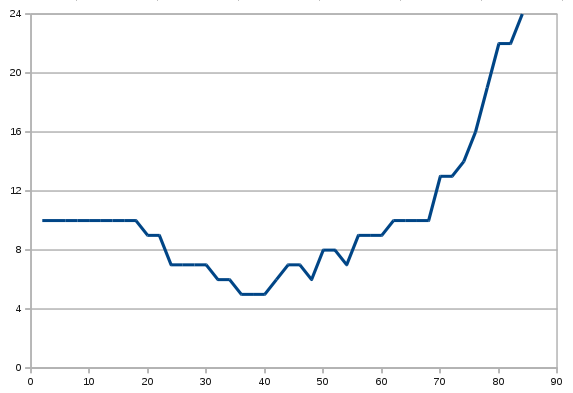
\includegraphics[width=\textwidth]{img/simul.png}
      \caption{Résultats d'une simulation de Risksim}
      \label{fig:simul}
    \end{figure}

    Sur un grand nombre de parties on peut constater que la probabilité pour le
    joueur rouge de gagner est de $50\%$.

  \section*{Deuxième partie}

    \subsection*{Grande armée ou armée rapide}

      \noindent
      Le nombre de planètes rouges est fixé à $70\%$ du nombre total de
      planètes.

      \begin{itemize}
        \item Lorsque le joueur bleu à un délai inter-attaque compris entre $7$
          à $12$ et $5$ à $10$ la probabilité que le joueur rouge gagne reste
          autour de $50\%$, augmentant légerement
        \item Lorsque le joueur bleu à un délai inter-attaque de $4$ à $9$ on
          constate que les probabilité que le joueur rouge gagne est de
          $65\%$
      \end{itemize}

      \medskip
      Nous pouvons donc conclure qu'une grande armée est plus efficace qu'une
      armée rapide.


    \subsection*{Grande armée ou armée très offensive}

      \noindent
      Le nombre de planètes rouges est fixé à $70\%$ du nombre total de
      planètes.

      \begin{itemize}
        \item Lorque le joueur bleu à un nombre de soldats attaquant égal à
      $60\%$ du nombre total de ses soldats, la probabilité que le joueur rouge
          gagne est de $30\%$
        \item Lorque le joueur bleu à un nombre de soldats attaquant égal à
      $65\%$ du nombre total de ses soldats, la probabilité que le joueur rouge
          gagne est de $25\%$
        \item Lorque le joueur bleu à un nombre de soldats attaquant égal à
      $70\%$ du nombre total de ses soldats, la probabilité que le joueur rouge
          gagne est de $19\%$
      \end{itemize}

      \medskip
      Nous pouvons donc conclure qu'une armée très offensive est plus efficace
      qu'une armée rapide. 


\end{document}
